% Created 2021-05-17 Mon 20:27
% Intended LaTeX compiler: pdflatex
\documentclass[presentation, 11pt,  aspectratio=169]{beamer}
\usepackage[utf8]{inputenc}
\usepackage[T1]{fontenc}
\usepackage{graphicx}
\usepackage{grffile}
\usepackage{longtable}
\usepackage{wrapfig}
\usepackage{rotating}
\usepackage[normalem]{ulem}
\usepackage{amsmath}
\usepackage{textcomp}
\usepackage{amssymb}
\usepackage{capt-of}
\usepackage{hyperref}
\usepackage{minted}
\setbeamertemplate{caption}{\raggedright\insertcaption\par}
\usepackage{tcolorbox}
\usepackage{etoolbox}
\BeforeBeginEnvironment{minted}{\begin{tcolorbox}[boxrule=0.5pt}%
\AfterEndEnvironment{minted}{\end{tcolorbox}}%
\hypersetup{colorlinks=false,linkbordercolor={0.2 0.2 0.3},urlbordercolor={0.8 0.8 0.8},pdfborderstyle={/S/U/W 0.5}}
\usetheme{Frankfurt}
\usecolortheme{orchid}
\author{Giovanni Moretti - giovanni@reflections.co.nz}
\date{\today}
\title{Gemini - a quieter web experience}
\subtitle{niceness through simplicity}
\AtBeginSection{\frame{\sectionpage}}
\hypersetup{
 pdfauthor={Giovanni Moretti - giovanni@reflections.co.nz},
 pdftitle={Gemini - a quieter web experience},
 pdfkeywords={},
 pdfsubject={},
 pdfcreator={Emacs 26.3 (Org mode 9.4.5)}, 
 pdflang={English}}
\begin{document}

\maketitle

\section*{State of the Web}
\label{sec:orgda71557}
\begin{frame}[label={sec:org555cada}]{The world-wide-web}
\begin{block}{Modern web browsers support dozens (hundreds) of standards}
\begin{itemize}
\item CSS\\
\item HTML 4, 5\\
\item Javascript\\
\item audio: .mp3 .ogg \ldots{}\\
\item graphics: .jpg .gif .png .svg \ldots{}\\
\item video display: .mp4 .webm \ldots{}\\
\item cookies\\
\item SSL encryption\\
\end{itemize}
\pause
\end{block}

\begin{block}{Resultant complexity is problematic}
\begin{itemize}
\item implausible to start from scratch\\
\item security and validation is difficult/impossible\\
\end{itemize}
\end{block}
\end{frame}

\begin{frame}[label={sec:org86f2207}]{Problems with WWW}
\begin{block}{User tracking}
\begin{itemize}
\item cookies, tracking pixels, browser fingerprinting\\
\end{itemize}
\end{block}

\begin{block}{Security is broken}
\begin{itemize}
\item too many (unknown) CAs trusted by default\\
\end{itemize}
\pause
\end{block}
\begin{block}{Pages heavy \& hard to know what's downloaded}
\begin{itemize}
\item DuckDuckGo: 26 requests - 1.3MB of content - 7 scripts\\
\item Google.com: 35 requests - 2.2MB of content - 11 scripts\\
\end{itemize}

\pause
\end{block}
\begin{block}{Layout \& formatting defined by the creator}
\begin{itemize}
\item lots on the screen at once -- distracting\\
\item page complexity and weight -- accessibility?\\
\end{itemize}
\end{block}
\end{frame}


\section*{Gemini}
\label{sec:orgca48a6f}
\begin{frame}[label={sec:org79edcb9}]{Gemini Overview}
\begin{block}{Started June 2019: Gemini is a new internet protocol that:}
\begin{itemize}
\item is heavier than gopher\\
\item is lighter than the web\\
\item will not replace either\\
\item strives for maximum power to weight ratio\\
\item takes user privacy very seriously\\
\end{itemize}
\pause
\end{block}

\begin{block}{Gemini Specifications}
\url{https://gemini.circumlunar.space/docs/specification.html}\\
\end{block}
\end{frame}


\begin{frame}[label={sec:org5c0a10f}]{Gemini Goals}
\begin{tiny}
FAQ: \href{gemini://gemini.circumlunar.space/docs/faq.gmi}{gemini://gemini.circumlunar.space/docs/faq.gmi}\\
\end{tiny}

\begin{block}{Gemini - a new application-level Internet protocol}
\begin{itemize}
\item for distributing of arbitrary files\\
\item a lightweight hypertext format\\
\end{itemize}
\end{block}

\begin{block}{Gemini is for people who are:}
\begin{itemize}
\item opposed to the web's ubiquitous tracking of users\\
\item tired of nagging pop-ups, obnoxious adverts, autoplaying videos\\
\item interested in low-power computing and/or low-speed networks\\
\end{itemize}
\pause
\end{block}
\begin{block}{You may think of Gemini as}
\begin{itemize}
\item "the web, stripped right back to its essence", OR\\
\item "Gopher, souped up and modernised just a little"\\
\end{itemize}
\end{block}
\end{frame}

\begin{frame}[label={sec:orgb0d32ef}]{Gopher - before the WWW}
\begin{columns}
\begin{column}{0.3\columnwidth}
\begin{block}{Gopher predates the web}
\begin{itemize}
\item created at Uni Wisconsin, Madison\\
\item intended to facilitate text search\\
\item links documents\\
\item used by libraries\\
\end{itemize}
\end{block}
\end{column}

\begin{column}{0.70\columnwidth}
\begin{center}
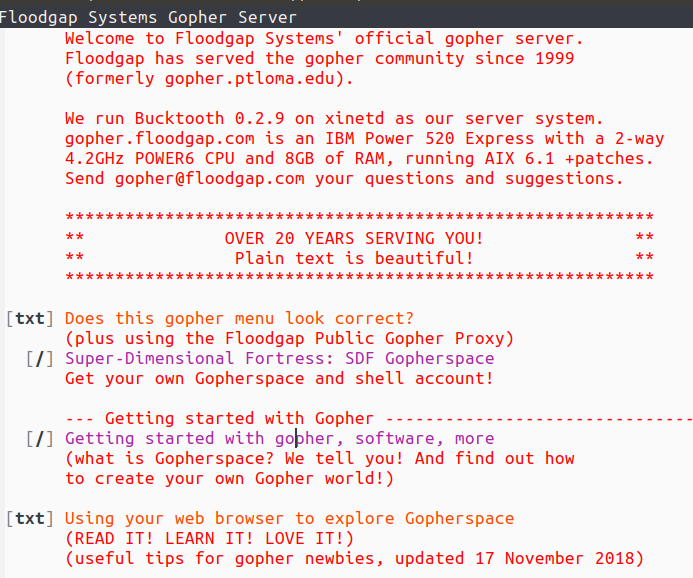
\includegraphics[height=0.85\textheight]{images/Gopher-1.png}
\end{center}
\end{column}
\end{columns}
\end{frame}


\begin{frame}[label={sec:orge5db9b4}]{Problems with Gopher}
\begin{itemize}
\item intended just for text\\
\item no support for other file types (images, video \ldots{})\\
\item no security (plain text transfer)\\
\end{itemize}
\pause
\begin{block}{Gemini has:}
\begin{itemize}
\item arbitrary non-ASCII character sets\\
\item linking to content in other protocols via simple URLs\\
\item identifies binary content using MIME types\\
\item redirects to prevent broken links\\
\item domain-based virtual hosting\\
\end{itemize}
\end{block}
\end{frame}

\begin{frame}[label={sec:org2aaf323}]{Gemini goals}
\begin{block}{Early Gemini discussion included three clear goals:}
\begin{enumerate}
\item it should be possible to remember the entire protocol spec\\
after reading it once or twice.\\

\item a basic but usable (not ultra-spartan) client should fit \\
in \(\approx\)50 lines of code in a modern language.\\

\item a client comfortable for daily use which implements every \\
single protocol feature should be a feasible weekend\\
project for a single developer.\\
\end{enumerate}
\pause
\end{block}
\begin{block}{It will be difficult to extend in the future}
so it \alert{stays} simple and privacy conscious\\
\end{block}
\end{frame}


\begin{frame}[label={sec:org408f758}]{Gemini - Text formatting}
\begin{itemize}
\item \alert{ALL} styling is done by the client\\
\item text lines will be wrapped\\
\item preformatted text is not altered or wrapped\\
\item UTF-8 is the default character set\\
\item there's no inline formatting: i.e. no bold/italics\\
\end{itemize}
\end{frame}

\begin{frame}[label={sec:org56261c7}]{Gemini clients control the page style}
\begin{figure}[htbp]
\centering
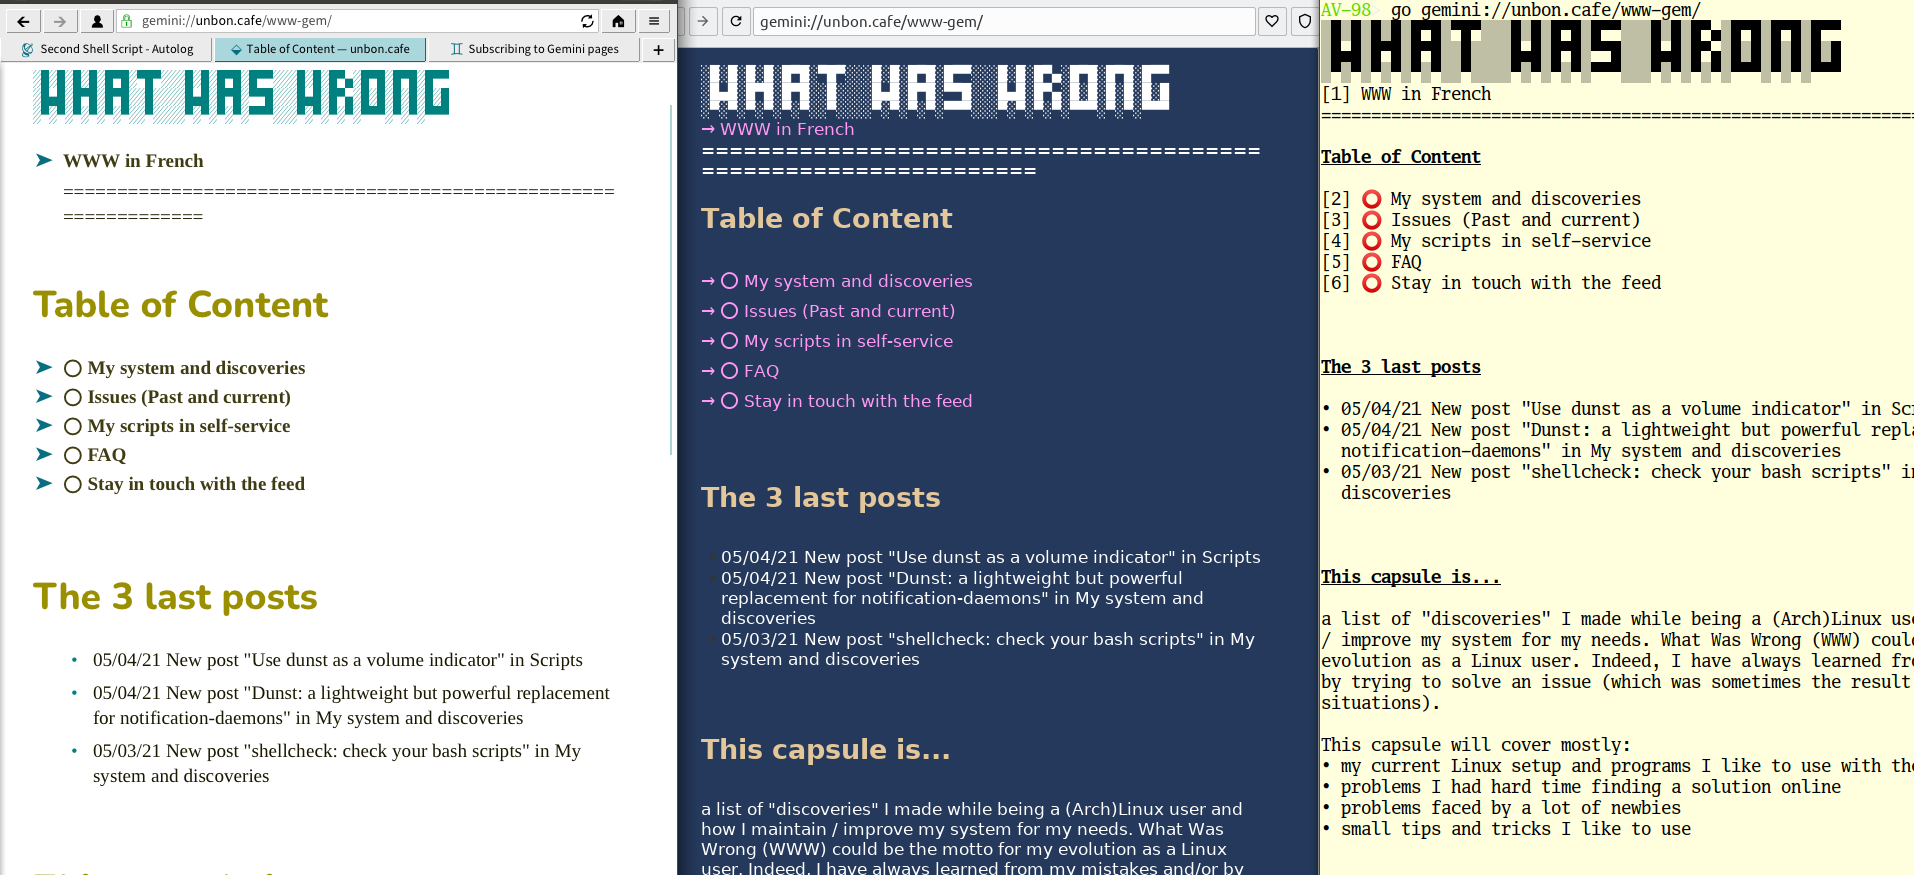
\includegraphics[width=1\textwidth]{images/threebrowsers.png}
\caption{Same page in Lagrange, Kristall and AV98 (terminal) browsers}
\end{figure}
\end{frame}

\begin{frame}[label={sec:org451e5b9}]{Gemini Markup}
\begin{block}{There are five core elements:}
\begin{itemize}
\item \alert{Headings:} start with '\#' '\#\#' or '\#\#\#'.\\
\begin{itemize}
\item level 1 header is usually page title.\\
\end{itemize}
\item \alert{List items:} begin with '*'\\
\item \alert{Quotes:} these lines begin with '>'\\
\item \alert{Preformatted text:} begins/ends with lines of three backticks (```)\\
\end{itemize}
\pause
\begin{itemize}
\item \alert{Links:} \emph{on a new line}, starting with \alert{=>}\\
=> \url{https://www.reddit.com} Reddit\\
=> image-dir/giant-peach.jpg\\
=> \href{gemini://gemini.circumlunar.space/docs/specification.gmi}{gemini://gemini.circumlunar.space/docs/specification.gmi}\\
=> \url{mailto:fred@example.com}\\
=> \href{gemini://podcast.com/episode-1.mp3}{gemini://podcast.com/episode-1.mp3}\\
\end{itemize}
\end{block}
\end{frame}


\begin{frame}[label={sec:org9524579}]{Why not use a subset of HTML?}
If the complexity of HTML is the problem, why not use a HTML subset:\\
\begin{itemize}
\item just headers, links and blockquote?\\
\end{itemize}

\pause
\begin{block}{Answered in FAQ (but briefly), using an HTML subset:}
\begin{enumerate}
\item you could never be sure what a server was sending\\
\begin{itemize}
\item you ask for one page: browser loads 30MB of images and 15 scripts \ldots{}\\
\end{itemize}
\item there's no clear delineation between Gemini and HTML sites\\
\item tracking/user profiling would still work\\
\item security of the (huge) browser still a problem\\
\end{enumerate}
\end{block}
\end{frame}

\begin{frame}[label={sec:org801b271}]{Let's see what Gemini users have created}
\begin{center}
\begin{tabular}{c}
Demo: let's explore Gemini Space\\
\end{tabular}
\end{center}
\end{frame}

\begin{frame}[label={sec:orgfd9c50d}]{What's the protocol: Gemini Request/Response}
\begin{quote}
A Gemini transaction: one request - one response:\\

\begin{enumerate}
\item Client: Opens connection\\
\item Server: Accepts connection\\
\item Client/Server: Complete TLS handshake\\
\item Client: Validates server certificate\\
\item \alert{Client: Sends one line Request-URL or URL+query-string)}\\
\item \alert{Server: Sends response header (one line), closes connection}\\
\item \alert{Server: Sends response body (text or binary data)}\\
\item Server: Closes connection\\
\item \alert{Client: Handles response}\\
\end{enumerate}
\end{quote}
\end{frame}

\begin{frame}[label={sec:orgb6a5140}]{Gemini Uploads are very limited}
Requests and response headers are limited to 1024 bytes\\

\begin{block}{After connecting, Return status '10' uploads data from client:}
\begin{quote}
\begin{center}
\begin{tabular}{ll}
 & \\
\hline
Client sends & \alert{\href{gemini://mysite.com/book-request.gmi}{gemini://mysite.com/book-request.gmi}}\\
Server responds & \alert{10 What Title:}\\
\hline
User enters & War and Peace\\
Client resends & \alert{\href{gemini://mysite.com/book-request.gmi?War\%20and\%20Peace}{gemini://mysite.com/book-request.gmi?War\%20and\%20Peace}}\\
\hline
server Responds & \alert{20 text/gemini; charset=utf-8}\\
 & The contents of War and Peace\\
\hline
\end{tabular}
\end{center}
\end{quote}
\end{block}
\end{frame}



\begin{frame}[label={sec:org638f154}]{TLS Certificate TOFU vs "Known" Validation}
\begin{block}{Gemini uses TLS v1.3 (ideally) or v1.2}
\begin{itemize}
\item no certificate authority required\\
\item users are based on "Trust on First Use" (TOFU) - like SSH\\
\end{itemize}

\pause
\end{block}
\begin{block}{Sites can identify returning users by their TLS certificate}
\begin{itemize}
\item no need for cookies for 'session persistence'\\
\item clients can support multiple certificates - user chooses\\
\item if a certificate is deleted, that identity is \emph{gone}\\
\end{itemize}
\end{block}
\end{frame}

\section*{Gemini Software}
\label{sec:orga67528b}
\begin{frame}[label={sec:org969f7eb}]{Gemini Servers}
Very little load on server - Raspberry Pi is fine\\

\begin{block}{Jetforce - written in Python 3}
\begin{itemize}
\item easy to set up\\
\item has CGI interface\\
\end{itemize}
\end{block}

\begin{block}{Agate - written in Rust}
\begin{itemize}
\item Installation: \href{gemini://gem.chriswere.uk/gemserver.gmi}{gemini://gem.chriswere.uk/gemserver.gmi}\\
\item or a video tutorial:\\
\end{itemize}
\begin{small}
\url{https://share.tube/videos/watch/4fe4e1f0-7896-4b8c-bfb8-2ff19c78d8e5}\\
\end{small}
\end{block}
\end{frame}

\begin{frame}[label={sec:org44a48e1}]{Gemini Browsers}
There's \emph{lots} of gemini software: \url{https://gemini.circumlunar.space/software/}\\

\begin{itemize}
\item \alert{Lagrange:} \url{https://github.com/skyjake/lagrange/releases/tag/v1.4.0}\\
\item \alert{Kristall:} \url{https://github.com/MasterQ32/kristall}\\
\item \alert{Amfora:} - terminal based client\\
\begin{itemize}
\item Playing with Gemini \& Amfora: \url{https://www.youtube.com/watch?v=i-iZ3R9U5ug}\\
\end{itemize}
\item \alert{Elpher} for Emacs - via Melpa\\
\item \alert{Android:} Ariane from Play Store\\
\item \alert{iPhone/Pad} Elaho from App Store and \url{https://github.com/pitr/gemini-ios}\\
\end{itemize}
\end{frame}

\begin{frame}[label={sec:orgbd0c8e6}]{Quick overview of Lagrange}
Lagrange is the most feature-rich Gemini browser:\\
\begin{itemize}
\item it looks really nice!\\
\item multiple tabs\\
\item subscriptions\\
\item inlining of images and audio\\
=> \href{gemini://fixato.org/2021-03-18-drawing-with-kiddos-crayons.gmi}{gemini://fixato.org/2021-03-18-drawing-with-kiddos-crayons.gmi}\\
\item clear certificate management\\
\item split-screen view\\
\item available for Linux, Mac and Windows\\
\end{itemize}
\end{frame}

\begin{frame}[label={sec:orga2d2346}]{Gemini's not just text:  Images loaded on request}
\begin{block}{Gemini's designer intended:}
\begin{itemize}
\item one request, one response: no hidden network activity\\
\item images can be inlined OR loaded in external viewer -- \alert{client decides}\\
\end{itemize}

\pause
\end{block}
\begin{block}{An example of a photo album in Gemini}
See\\
\begin{small}
\begin{itemize}
\item \href{gemini://fixato.org/2021-03-10-eye-of-fixato-an-example-photo-album-for-gemini.gmi}{gemini://fixato.org/2021-03-10-eye-of-fixato-an-example-photo-album-for-gemini.gmi}\\
\end{itemize}
\end{small}
It has\\
\begin{itemize}
\item one image as an index\\
\item detailed descriptions, which are good for accessibility\\
\end{itemize}
\end{block}
\end{frame}



\section*{"Built on Gemini"}
\label{sec:org5daeb9f}
\begin{frame}[label={sec:orgcc90025}]{Subscribing to Gemini pages}
Options: Browser detects change in page headings OR simple day-timestamp scheme:\\
\begin{footnotesize}
\begin{quote}
Welcome to my Gemlog, where you can read every Friday about my adventures in urban gardening and abstract algebra!\\

\#\# My posts\\
=> \alert{bokashi.gmi              2020-11-20 - Early Bokashi composting experiments}\\
=> \alert{finite-simple-groups.gmi 2020-11-13 - Trying to get to grips with finite simple groups\ldots{}}\\
=> \alert{balcony.gmi              2020-11-06 - I started a balcony garden!}\\

\#\# Other gemlogs I enjoy\\
=> \href{gemini://example.com/foo/}{gemini://example.com/foo/}    Abelard Lindsay's gemlog\\
=> \href{gemini://example.net/bar/}{gemini://example.net/bar/}    Vladimir Harkonnen's gemlog\\
=> \href{gemini://example.org/baz/}{gemini://example.org/baz/}    Case Pollard's gemlog\\
\end{quote}
\end{footnotesize}
from \href{gemini://gemini.circumlunar.space/docs/companion/subscription.gmi}{gemini://gemini.circumlunar.space/docs/companion/subscription.gmi}\\
\end{frame}

\begin{frame}[label={sec:org0fb3997}]{What are people doing with it?}
Lots\\
\begin{itemize}
\item \alert{Gemini-to-Web proxy} - \url{https://portal.mozz.us}\\
\item \alert{Gemini Quickstart} - \href{gemini://geminiquickst.art/}{gemini://geminiquickst.art/}\\
\item \alert{Gemini Search:} \href{gemini://geminispace.info}{gemini://geminispace.info}\\
\item \alert{Geminispace aggregator} - \href{gemini://gemini.circumlunar.space/capcom}{gemini://gemini.circumlunar.space/capcom}\\
\item \alert{TrouserMonkey.net} -- \href{gemini://trousermonkey.net}{gemini://trousermonkey.net}\\
\item \alert{Blogging Client in 30 lines} \\
-- \href{gemini://spool-five.com/gemlog/2021-04-01-second_script.gmi}{gemini://spool-five.com/gemlog/2021-04-01-second_script.gmi}\\
\item \alert{Blogging} -- \href{gemini://fixato.org/2020-03-25-an-uneventful-day.gmi}{gemini://fixato.org/2020-03-25-an-uneventful-day.gmi}\\
\item \alert{Podcasts} -- \href{gemini://gem.chriswere.uk/trendytalk/}{gemini://gem.chriswere.uk/trendytalk/}\\
\item \alert{Proxying other services:}\\
\begin{itemize}
\item HackerNews - \url{https://news.ycombinator.com/item?id=25986378}\\
\end{itemize}
\end{itemize}

Mastodon: \url{https://mastodon.social/tags/gemini}\\
\end{frame}

\begin{frame}[label={sec:orgdc59568}]{Small Web (smolweb) related sites}
\begin{itemize}
\item \alert{Tilde sites:} e.g.\\
\begin{itemize}
\item \url{https://tildeverse.org/} \\
\item \url{https://tilde.team/} \\
\item \href{gemini://tilde.team}{gemini://tilde.team}  -- Free Gemini Hosting\\
\end{itemize}
\item \alert{Pubnixes:} Public Unix servers\\
Super Dimensional Fortress:\\
\begin{itemize}
\item \url{https://sdf.org}\\
\item \url{https://sdfeu.org}\\
\end{itemize}
\end{itemize}
\end{frame}

\begin{frame}[label={sec:orgf264ee5}]{Interesting Gemini sites}
\begin{itemize}
\item \alert{Konpeito is quarterly Lo-fi hip-hop \& chill mixtape} - \href{gemini://konpeito.media}{gemini://konpeito.media}\\
\item \alert{xj9 - tech blog} \href{gemini://sunshinegardens.org/~xj9}{gemini://sunshinegardens.org/~xj9}\\
\item \alert{Sunshine Gardens:} \href{gemini://sunshinegardens.org}{gemini://sunshinegardens.org}\\
\item \alert{How I use RSS:} \href{gemini://gemlog.blue/users/joelchrono12/1612624540.gmi}{gemini://gemlog.blue/users/joelchrono12/1612624540.gmi} \\
\item \alert{Progress to Offline first:} -\\
\begin{small} gemini://gemini.circumlunar.space/~solderpunk/gemlog/progress-toward-offline-first.gmi
\end{small}
\item \alert{News sites proxied to Gemini:} \href{gemini://simplynews.metalune.xyz}{gemini://simplynews.metalune.xyz}\\
\item \alert{One Hundred Rabbits (resilience, offline-first, sailing, cooking, Plan9, design):}$\backslash$\ \href{gemini://gemini.circumlunar.space/users/hundredrabbits}{gemini://gemini.circumlunar.space/users/hundredrabbits}\\
\item \alert{Gembooks \& .gpub - an eBook format using Gemini:}\\
\begin{itemize}
\item \url{https://codeberg.org/oppenlab/gempub}\\
\end{itemize}
\end{itemize}
\end{frame}

\begin{frame}[label={sec:orgf254bcb}]{Conclusion}
\begin{block}{Gemini}
\begin{itemize}
\item \alert{for users}\\
\begin{itemize}
\item provides very simple and accessible markup for creating pages\\
\item is suitable for many (but not all) documents\\
\item provides an ad-free, secure, and distraction-free environment\\
\item provides a human-scale community of users\\
\end{itemize}

\item \alert{for developers}\\
\begin{itemize}
\item is simple enough to encourage experimentation\\
\item simple gemtext markup is easily mapped to other formats\\
\item has low hardware and network traffic requirements\\
\end{itemize}
\end{itemize}
\end{block}
\begin{block}{}
\begin{center}
\begin{tabular}{c}
QUESTIONS?\\
\end{tabular}
\end{center}
\end{block}
\end{frame}
\begin{frame}[label={sec:org9cfb259}]{Links \& Reuse/License}
\begin{block}{Links}
\begin{itemize}
\item \alert{Getting Started with Gemini:} \href{gemini://geminiquickst.art}{gemini://geminiquickst.art} \(\leftarrow\) \alert{Really Good}\\
\item \alert{Gemini Home:} \url{https://gemini.circumlunar.space}\\
\item \alert{Gemini Search:} \href{gemini://geminispace.info}{gemini://geminispace.info}\\
\item \alert{Gemini on Mastodon:} \url{https://mastodon.social/web/timelines/tag/gemini}\\
\end{itemize}
\end{block}

\begin{block}{Reuse this presentation}
\begin{center}

\includegraphics[width=0.25\textwidth]{images-external/cc-by-sa.png}
\end{center}

\begin{small}
This presentation is Copyright (C) 2021 Giovanni Moretti.\\

This work is licensed under a Creative Commons Attribution-ShareAlike 4.0 International License. For more information, go to\\
~~ \url{http://creativecommons.org/licenses/by-sa/4.0/}\\
\end{small}
\end{block}
\end{frame}
\end{document}